\newpage
\section{Aufbau und Durchführung}
\subsection{Aufbau}
\label{sec:Aufbau}
    \begin{figure}[ht]
        \centering\captionsetup{format=plain}
        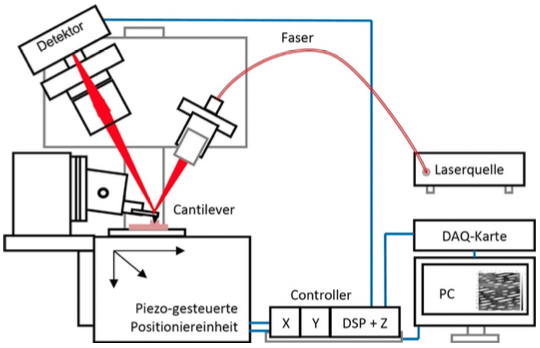
\includegraphics[width=0.6\textwidth]{bilder/Aufbau.png}
        \caption{Hier ist der schematische Aufbau des benutzten AFM dargestellt. \cite{anleitung}}
        \label{fig:Aufbau}
    \end{figure}
    \FloatBarrier
    In diesem Aufbau wird die Probe in x-,y-,z-Richtung durch grobe und feine Justierschrauben und durch piezoelektrische Elemente bewegt.
    Zur Detektion der Auslenkung des Cantilevers wird die Laserreflektionsmethode verwendet.
    Dazu wird ein Faserlaser der Wellenlänge $\SI{635}{nm}$ auf die spiegelnde Rückseite des Cantilevers fokussiert und auf eine Viersegment-Photodiode reflektiert.
    Das Signal des Detektors wird dazu benutzt die Auslenkung des Cantilevers über eine Closed-Loop konstant zu halten, die die z-Position der Probe nachregelt.
    Die Probe wird mithilfe der Piezoelemente abgerastert und die Bewegung der Probe wird an jeden Punkt als Höheninformation aufgenommen.
    Dehnungsmessstreifen an den Piezoelementen in der xy-Ebene messen die genaue laterale Position der Probe und stellen somit sicher, dass die in \autoref{sec:piezo} besprochenen Störungen keine Auswirkung auf die gemessenen AFM-Bilder haben.

\subsection{Durchführung}
\label{sec:Durchfuehrung}
    Die Prozedur zum Messen des AFM-Bildes ist für alle benutzten Proben gleich.
    Zuerst wird die Probe mit einer Pinzette möglichst auf die Mitte der Stage gelegt.
    Die Stage ist dabei so weit wie möglich von der Spitze entfernt um diese nicht aus Versehen zu beschädigen.
    Danach wird die Grobjustierschraube benutzt, um die Probe so nah an die Spitze anzunähern, dass der Abstand mit dem bloßen Auge nicht mehr zu erkennen ist.
    Im Anschluss daran wird langsam an der Feinjustierschraube gedreht, bis auf der der Laserspot in der Software der Viersegment-Photodiode in den Ursprung springt.
    Bei angeschalteter Nachregelung wird so lange weitergedreht, dass die Spannung des z-Piezoelements \SI{25}{V} anzeigt, sodass die Spannung im Intervall $[0,50]\,$V variiert werden kann.
    Es wurden immer Scans mit wenigen Rasterpunkten und hoher Scangeschwindigkeit durchgeführt, damit man einen Überblick über den betrachteten Scanbereich bekam und die jeweils gesuchte Struktur schnell gefunden werden konnte.

    Als Erstes sollten $20 \times 20\, \mu$m große Teilbereiche einer bekannten Mikrostruktur gemessen werden mit den Scanparametern $250 \times 250$ Pixel und der Scangeschwindigkeit $100$Pixel/s.
    Dann wurden Bilder eines Teils einer CD [$10 \times 10\, \mu$m, $250 \times 250$ Pixel, $100$Pixel/s], einer DVD [$5 \times 5\, \mu$m, $250 \times 250$ Pixel, $100$Pixel/s] und einer Bluray [$2 \times 2\, \mu$m, $250 \times 250$ Pixel, $50$Pixel/s] aufgenommen.
    Als Letztes werden mehrere Kraft-Abstands-Kurven für verschiedene Materialien gemessen.
    Dazu wurde die Nachregelung des z-Piezos ausgestellt.